\section{Auswertung} 

\subsection{Strömungsgeschwindigkeit aus der Dopplerverschiebung}

\begin{align}
    \intertext{Im ersten Teil der Versuchsreihe wird die Strömungsgeschwindigkeit an einem Rohr mit einem Innendurchmesser von $10\,\unit{\milli\meter}$, mit Hilfe des Impuls-Echo-Verfahren, bestimmt. 
    Dabei wird das Ultraschallgerät an drei verschiedene Einstellwinkel angesetzt (15\unit{\degree}, 30\unit{\degree}, 45\unit{\degree}). 
    Zuvor berechnet sich der Dopplerwinkel $\alpha$ mit der Formel (\ref{5}). }
    \alpha_{15\unit{\degree}} = 80,06\unit{\degree} \notag \\
    \alpha_{30\unit{\degree}} = 70,52\unit{\degree} \notag \\
    \alpha_{45\unit{\degree}} = 61,87\unit{\degree} \notag
    \intertext{Demnach wird die Strömungsgeschwindigkeit für fünf verschiedene Flussgeschwindigkeiten für alle drei Dopplerwinkel durchgeführt.
    Die Voreinstellung der Sonde beträgt $2\,\unit{\mega\hertz}$.
    Die Frequenzverschiebung sowie flow und speed werden tabellarisch festgehalten in der Tabelle \ref{Tabelle3}, \ref{Tabelle4} und \ref{Tabelle5}.
    Die theoretische Strömungsgeschwindigkeit berechnet sich durch die Formel (\ref{4}), durch das Umformen folgt:}
    \text{v} = \frac{\increment \nu \cdot \text{c}}{2 \cdot \nu_{0} \cos \alpha}. 
    \intertext{Die errechneten Strömungsgeschwindigkeiten von den drei verschiedenen Winkeln werden mit den Theoriewerten, welche sich durch die Formel}
    \text{v} = \frac{\dot{v}}{\pi \cdot \text{R}^2 }
    \intertext{errechnen lässt, verglichen.} \notag
\end{align}

\begin{table}[H]  
    \centering
    \caption{Theoriewerte zu den Flussgeschwindigkeiten.} 
    \label{Tabelle2}
    \begin{tabular} {c  c  c  c}
        \toprule
        {$ \text{Flussgeschwindigkeit} \mathbin{/} \frac{\text{l}}{\text{min}} $} &
        {$ \text{v}_{\text{theo}} \mathbin{/} \frac{\unit{\meter}}{\unit{\second}}  $} \\
        \midrule
        3,0 & 0.63 \\
        3.5 & 0.74 \\
        4.0 & 0.85 \\
        4.5 & 0.95 \\
        5.0 & 1.06 \\
        \bottomrule
    \end{tabular} 
\end{table}

\begin{table}[H]
    \centering
    \caption{Die Messwerte des ersten Arbeitsauftrages für den Winkel $15\unit{\degree}$} 
    \label{Tabelle3}
    \begin{tabular} {c  c  c  c  c  c} 
        \toprule
        {$ \text{Pumprate} \mathbin{/} \frac{\unit{\liter}}{\unit{\minute}} $} &
        {$ \increment \nu \mathbin{/} \unit{\hertz} $} &
        {$ \text{speed} \mathbin{/} \frac{\unit{\meter}}{\unit{\second}} $} &
        {$ \text{flow} \mathbin{/} \frac{\unit{\liter}}{\unit{\minute}} $}&
        {$ \text{v} \mathbin{/} \frac{\text{m}}{\text{s}} $} &
        {$ \frac{\increment \nu}{\cos \alpha} $} \\
        \midrule
        3,0 & 190 & 2,39 & 1,1 & 0,49 & 1100,70 \\
        3,5 & 161 & 2,12 & 1,0 & 0,41 & 932,70  \\
        4,0 & 281 & 3,45 & 1,6 & 0,73 & 1627,88 \\
        4,5 & 243 & 2,65 & 1,2 & 0,46 & 1407,74 \\
        5,0 & 404 & 4,48 & 2,3 & 1,05 & 2340,44 \\
        \bottomrule
    \end{tabular} 
\end{table}

\begin{table}[H]
    \centering
    \caption{Die Messwerte des ersten Arbeitsauftrages für den Winkel $30\unit{\degree}$} 
    \label{Tabelle4}
    \begin{tabular} {c  c  c  c  c  c}
        \toprule
        {$ \text{Pumprate} \mathbin{/} \frac{\unit{\liter}}{\unit{\minute}} $} &
        {$ \increment \nu \mathbin{/} \unit{\hertz} $} &
        {$ \text{speed} \mathbin{/} \frac{\unit{\meter}}{\unit{\second}} $} &
        {$ \text{flow} \mathbin{/} \frac{\unit{\liter}}{\unit{\minute}} $} &
        {$ \text{v} \mathbin{/} \frac{\text{m}}{\text{s}} $} &
        {$ \frac{\increment \nu}{\cos \alpha} $} \\
        \midrule
        3,0 & 605  & 3,71 & 1,7 & 0,81 & 1814,21 \\
        3,5 & 607  & 4,12 & 1,9 & 0,81 & 1820,21 \\
        4,0 & 898  & 5,77 & 2,7 & 1,21 & 2692,83 \\
        4,5 & 904  & 6,01 & 2,8 & 1,21 & 2710,82 \\
        5,0 & 1270 & 8,38 & 4,0 & 1,71 & 3808,34 \\
        \bottomrule
    \end{tabular} 
\end{table}

\begin{table}[H]
    \centering
    \caption{Die Messwerte des ersten Arbeitsauftrages für den Winkel $45\unit{\degree}$} 
    \label{Tabelle5}
    \begin{tabular} {c  c  c  c  c  c}
        \toprule
        {$ \text{Pumprate} \mathbin{/} \frac{\unit{\liter}}{\unit{\minute}} $} &
        {$ \increment \nu \mathbin{/} \unit{\hertz} $} &
        {$ \text{speed} \mathbin{/} \frac{\unit{\meter}}{\unit{\second}} $} &
        {$ \text{flow} \mathbin{/} \frac{\unit{\liter}}{\unit{\minute}} $} &
        {$ \text{v} \mathbin{/} \frac{\text{m}}{\text{s}} $} &
        {$ \frac{\increment \nu}{\cos \alpha} $} \\
        \midrule
        3,0 & 324 & 1,55 & 0,7 & 0,31 & 687,20 \\
        3,5 & 412 & 1,94 & 0,9 & 0,39 & 873,85 \\
        4,0 & 506 & 2,23 & 1,1 & 0,48 & 1073,23 \\
        4,5 & 631 & 3,01 & 1,4 & 0,60 & 1338,35 \\
        5,0 & 698 & 3,11 & 1,5 & 0,66 & 1480,46 \\
        \bottomrule
    \end{tabular} 
\end{table}

\begin{align*}
    \intertext{Daraus folgt}
    \nu_{15\unit{\degree}} = (0,459\pm 0,303)\,\frac{\text{m}}{\text{s}} \\
    \nu_{30\unit{\degree}} = ( 1,150 \pm 0,371 )\,\frac{\text{m}}{\text{s}} \\
    \nu_{45\unit{\degree}} = ( 0,488 \pm 0,128 )\,\frac{\text{m}}{\text{s}}.
    \intertext{Zudem wird das Verhältnis $\frac{\increment \nu}{\cos \alpha}$ gegen die errechneten Strömungsgeschwindigkeiten der drei Dopplerwinkel geplottet.} 
\end{align*}

\begin{figure}[H]
    \centering
    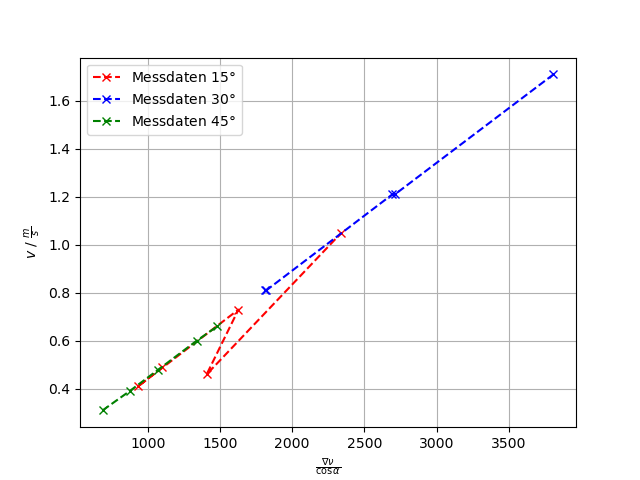
\includegraphics[height=80mm]{bilder/Plot1.png}
    \caption{Geschwindigkeit gegen das Verhältnis der Dopplerwinkel.\label{Abbildung2} }
\end{figure}

\begin{flushleft}
    Wie zu beobachten, steigen die Geschwindigkeiten bei zunehmenden Verhältnis linear.
    Die Messdaten für $30\unit{\degree}$ sowie $45\unit{\degree}$ liegen mehrfach auf der Gerade, wohingegen bei $15\unit{\degree}$ einige Abweichungen vorhanden sind.
\end{flushleft}

\subsection{Strömungsgeschwindigkeit und Streuintensität in Abhängigkeit der Messtiefe}

\begin{flushleft}
    Im nächsten Teil der Versuchsreihe wird die Flussgeschwindigkeit auf 70\% der maximalen Leistung des Gerätes gebracht welche $5,2\,\frac{l}{\text{min}}$ entspricht.
    Es wird mit einem Einstellwinkel von $15\unit{\degree}$ und einem Rohrdurchmesser von $10\,\unit{\milli\meter}$ durchgeführt.
    Die Messtiefe beginnt bei $12\,\unit{\micro\meter}$ und wird in $0,5\,\unit{\micro\meter}$ bis $18\,\unit{\micro\meter}$ gemessen.
    Dies entspricht einer Messtiefe von $11\,\unit{\milli\meter}$ bis $30\,\unit{\milli\meter}$.
    Die Streuintensität sowie die Strömungsgeschwindigkeit werden in Abhängigkeit der Messtiefe werden in der Tabelle \ref{Tabelle6} festgehalten.
\end{flushleft}

\begin{table}[H]
    \centering
    \caption{Die Messwerte des zweiten Arbeitsauftrages für 45\% der maximal Pumpleistung} 
    \label{Tabelle6}
    \begin{tabular} {c  c  c  c  c}
        \toprule
        {$ \text{Messtiefe} $} &
        {$ \increment \nu \mathbin{/} \unit{\hertz} $} &
        {$ \text{Intensität} \mathbin{/} 1000 \cdot \frac{\text{V}^2}{\unit{\second}} $} &
        {$ \text{v} \mathbin{/} \frac{\text{m}}{\text{s}} $} \\
        \midrule
        12,5 & 479 & 61   & 1,24 \\
        13,0 & 583 & 87   & 1,51 \\
        13,5 & 623 & 102  & 1,62 \\
        14,0 & 663 & 131  & 1,72 \\
        14,5 & 680 & 140  & 1,77 \\
        15,0 & 675 & 161  & 1,75 \\
        15,5 & 625 & 177  & 1,62 \\
        16,0 & 546 & 190  & 1,42 \\
        16,5 & 480 & 145  & 1,25 \\
        17,0 & 466 & 130  & 1,21 \\
        17,5 & 560 & 115  & 1,45 \\
        18,0 & 568 & 98   & 1,48 \\
        18,5 & 599 & 92   & 1,56 \\
        \bottomrule
    \end{tabular} 
\end{table}



\begin{flushleft}
    Die Durchführung wird wiederholt für 45\% der maximalen Leistung des Gerätes anschließend die Messwerte in Tabelle \ref{Tabelle7} festgehalten.
\end{flushleft}

\begin{table}[H]
    \centering
    \caption{Die Messwerte des zweiten Arbeitsauftrages für 70\% der maximal Pumpleistung} 
    \label{Tabelle7}
    \begin{tabular} {c  c  c  c}
        \toprule
        {$ \text{Messtiefe} $} &
        {$ \increment \nu \mathbin{/} \unit{\hertz} $} &
        {$ \text{Intensität} \mathbin{/} 1000 \cdot \frac{\text{V}^2}{\unit{\second}} $} &
        {$ \text{v} \mathbin{/} \frac{\text{m}}{\text{s}} $} \\
        \midrule
        12,5 & 244 & 53  & 0,63 \\
        13,0 & 281 & 79  & 0,73 \\
        13,5 & 299 & 91  & 0,77 \\
        14,0 & 319 & 122 & 0,83 \\
        14,5 & 317 & 115 & 0,82 \\
        15,0 & 304 & 170 & 0,79 \\
        15,5 & 287 & 120 & 0,74 \\
        16,0 & 247 & 114 & 0,64 \\
        16,5 & 224 & 71  & 0,58 \\
        17,0 & 235 & 73  & 0,61 \\
        17,5 & 251 & 65  & 0,65 \\
        18,0 & 266 & 92  & 0,69 \\
        18,5 & 259 & 112 & 0,67 \\
        \bottomrule
    \end{tabular} 
\end{table}

\begin{flushleft}
    Daraufhin werden die Geschwindigkeiten und Streuintensitäten der einzelnen Messtiefe in einem Diagramm in Abhängigkeit der Messtiefe dargestellt.
\end{flushleft}

\begin{figure}[H]
    \centering
    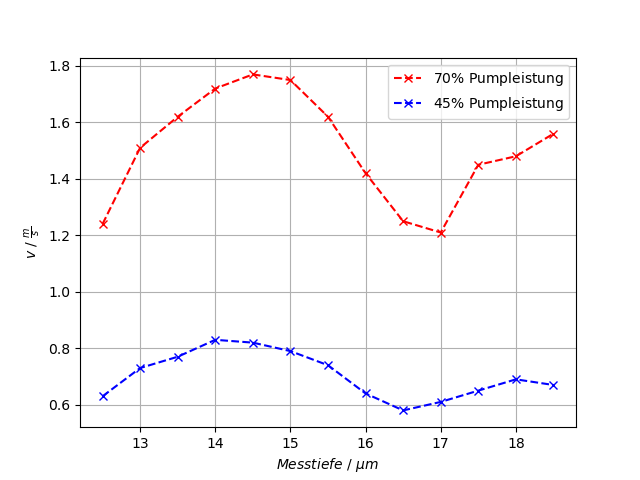
\includegraphics[height=80mm]{bilder/Plot3.png}
    \caption{Die Geschwindigkeiten gegen die Messtiefe geplottet.\label{Abbildung3} }
\end{figure}

\begin{figure}[H]
    \centering
    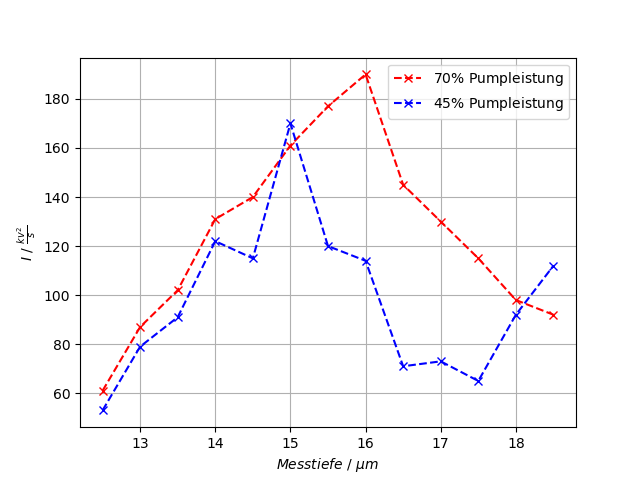
\includegraphics[height=80mm]{bilder/Plot4.png}
    \caption{Die Intensität gegen die Messtiefe geplottet.\label{Abbildung4} }
\end{figure}

\begin{flushleft}
    Im Diagramm \ref{Abbildung3} ist es zu erkennen, dass die Geschwindigkeit der höheren Leistung deutlich größer sind.
    Zudem zeigt sich bei beiden eine Wellenartige Funktion, die durch das Absenden der Impulse erklären lässt.
    Je tiefer die Messtiefe ist, desto größer die Wartezeit zwischen den Impulsen.
    Am Anfang ist der Sendeimpuls klein und wird größer mit zunehmender Messtiefe.
    Dazu kommt noch ein Schallimpuls, für Hin- und Rückweg, was dafür sorgt, dass die Funktion wellenartig wird.
    Diese Deutung kann ebenso auf das Diagramm \ref{Abbildung4} hergeleitet werden, wobei eine größere Messung mit mehr Messtiefen benötigt wird. 
\end{flushleft}